\documentclass[10pt,a4paper]{article}
\usepackage{amsmath}
\usepackage{amsfonts}
\usepackage{amssymb}
\usepackage{graphicx}
\usepackage{multicol}
\usepackage{tabularx}
\usepackage{tikz}
\usetikzlibrary{arrows,shapes,automata,petri,positioning,calc}
\usepackage{hyperref}
\usepackage{tikz}
\usepackage{gensymb}
\usepackage{polynom}
\usetikzlibrary{matrix,calc}
\makeatletter
\newcommand\xleftrightarrow[2][]{%
  \ext@arrow 9999{\longleftrightarrowfill@}{#1}{#2}}
\newcommand\longleftrightarrowfill@{%
  \arrowfill@\leftarrow\relbar\rightarrow}
\makeatother
\usepackage[margin=0.5in]{geometry}
\newcommand{\myvec}[1]{\ensuremath{\begin{pmatrix}#1\end{pmatrix}}}
\let\vec\mathbf
\newenvironment{Figure}
  {\par\medskip\noindent\minipage{\linewidth}}
  {\endminipage\par\medskip}
\begin{document}
%--------------------logo figure-------------------------%
\begin{figure*}[!tbp]
 \centering
  \begin{minipage}[b]{0.4\textwidth}
  
\includegraphics[scale=.25]{iitlogo.png} 
  \end{minipage}
\end{figure*}
%--------------------name & rollno-----------------------
\raggedright \textbf{Name}:\hspace{1mm} Ganga Gopinath\hspace{3cm} \Large \textbf{Matrix Assignment}\hspace{2.5cm} % 
\normalsize \textbf{Roll No.} :\hspace{1mm} FWC22050\vspace{1cm}
\begin{multicols}{2}
\section{Problem statement:}  Construct a triangle PQR in which QR=6cm, $\angle{Q}=60^0$ and PR - PQ = 2cm.\vspace{3mm}


\textbf{Law of Cosines}
\vspace{2mm}\raggedright \\

The law of Cosines relates the length of the triangle to the cosines of one of its angles. It states that, if the length of two sides and the angle between them is known for a triangle, then we can determine the length of the third side. It is given by:
\begin{equation}
	\vec{q}^2=\vec{p}^2+\vec{r}^2-
\vec{2prcos \theta} 
 \end{equation}

%-----------------------------solution---------------------------
\raggedright \textbf{SOLUTION}:\vspace{5mm}\\
\raggedright \textbf{Steps of Construction:}\vspace{2mm}\\
\textbf{Step 1:}\vspace{2mm}\\
Let P,Q and R be the vertices of the triangle  with coordinates.

Given QR length is a=6cm,
So the coordinates of vertices  Q,R and P are :\vspace{2mm}\\
\begin{center}$
\vec{
 Q =\begin{pmatrix}
0 \\
0 
\end{pmatrix} 
\vspace{1mm}
R=\begin{pmatrix}
6 \\
0 
\end{pmatrix} 
\vspace{1mm}
P=r\begin{pmatrix}
sin \theta\\
  cos \theta\\
\end{pmatrix} }
\vspace{1mm}$
\end{center}
Also given the angle is $Q=60^0$,so by finding the coordinates of the other sid
    e we can form a required triangle. \\
 \vspace{2mm}
For the input parameters in Table 1.\\
{\setlength\extrarowheight{2pt}
\begin{center}
\begin{tabular}{|c|c|c|}
	\hline
	\textbf{Symbol}&\textbf{Value}&\textbf{Description}\\
	\hline
	Q&$\begin{pmatrix}
	0\\0\\
	\end{pmatrix} $& Q Point\\
	\hline
	R&$\begin{pmatrix}
	6\\0\\
	\end{pmatrix} $& R Point\\
	\hline
	$\theta$&60$^{\circ}$&$\angle$PQR\\
	\hline
	r-q & 2 & PR-PQ\\
	\hline
	r&  & PR\\
	\hline
	q &  & PQ\\
	\hline
	p & 6 & QR\\
	\hline
\end{tabular}
%}\\
\\ {Table 1}\\
\end{center}
\vspace{3mm} 
By using the Cosine formula in  $\Delta$PQR \\ 
\begin{equation}
	\vec{q}^2=\vec{p}^2+\vec{r}^2-
\vec{2prcos\theta} 
\end{equation}
\begin{center}
	$0=p^2+r^2 -q^2-2prcos\theta$\\
\vspace{5mm}

0=(r+q)(r-q)+${6}^2$ - 2 $\times$ 6 $\times$ .5r\\
\vspace{5mm}
\end{center}
After simplification
\begin{equation}
	   2r-q =18
\end{equation}
Given that,
\begin{equation}
	r-q=2
\end{equation}
\textbf{Step 2:}\vspace{2mm}\\

Using equation (3) and (4),
\begin{equation}
  \begin{pmatrix}
2 & -1\\
1 &-1
\end{pmatrix} 
\begin{pmatrix}
r\\
q
\end{pmatrix} 
=
\begin{pmatrix}
18 \\ 
 2\
\end{pmatrix}
\end{equation}\vspace{2mm}\\


The augmented matrix for the above matrix equation is 
\vspace{3mm}
\begin{equation}
\begin{pmatrix}
  2 & -1 & \vrule & 18\\
  1 & -1  &\vrule & 2
    \end{pmatrix}  
    \end{equation}
    \begin{center}
   $\xleftrightarrow{\text{$R_1$ $\leftarrow  \frac{R_1}{2}$}}$
$ \begin{pmatrix}
  1 & \frac{-1}{2} & \vrule & 9\\
 1 & -1  &\vrule & 2	  
  \end{pmatrix}$ \\
   \end{center}
   \begin{center}
$ \xleftrightarrow{\text{$R_2$ $\leftarrow  {R_2}-{R_1}$}} $
$\begin{pmatrix}
 1 & - \frac{1}{2} & \vrule & 9\\
  0 & -\frac{1}{2}  &\vrule & 14\
  \end{pmatrix}$
  \\
  \end{center}
  \begin{center}
  $ \xleftrightarrow{\text{$R_1$ $\leftarrow  \frac{R_2}{\frac{-1}{2}}$}} $
$\begin{pmatrix}
  1 & 0 & \vrule & 16\\
  0 & 1  &\vrule & 14\
  \end{pmatrix}$
  \\
  \end{center}
  \begin{equation}
\implies X = 
   \begin{pmatrix}
   16 \\ 14
 \end{pmatrix}
 \end{equation}
Using equation (7) we get ,
\begin{equation}
	r = 16 \vspace{2mm}
\end{equation}
\begin{equation}
	q = 14 \vspace{2mm}
\end{equation}
The vertices of $\Delta$ PQR are \\
\begin{equation}
p= 16 \begin{pmatrix}
cos 60\\
sin 60\\
\end{pmatrix} 
,Q= \begin{pmatrix}
 0\\
 0\\
 \end{pmatrix} 
,R= \begin{pmatrix}
 6\\
 0\\
\end{pmatrix} 
\end{equation} \vspace{2mm}


\textbf{Result} 
\begin{center}
	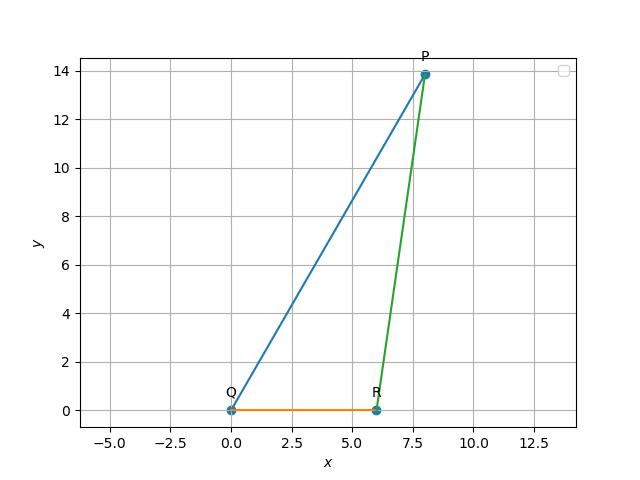
\includegraphics[width=0.4\textwidth]{ex2.jpg}
\end{center}\vspace{5mm}
\newpage
\vspace{4mm}  
\textbf{Implementation}
\begin{center}
\setlength{\arrayrulewidth}{0.5mm}
\setlength{\tabcolsep}{5pt}
\renewcommand{\arraystretch}{3}
    \begin{tabular}{|l|c|}
    \hline 
    \textbf{Equation no} & \textbf{Role} \\ \hline
    1 &  law of Cosines \\ 
    5 & Matrix form of Linear equation  \\
    %10 & Results Identity matrix  \\
    8 & Length of r\\
    9 & Length of q \\
    
    \hline
      \end{tabular}
  \end{center} \vspace{2mm} 



  \vspace{2mm} \textbf{Construction}
\begin{center}
\setlength{\arrayrulewidth}{0.5mm}
\setlength{\tabcolsep}{6pt}
\renewcommand{\arraystretch}{1.5}
    \begin{tabular}{|l|c|}
  \hline 
  \textbf{vertex} & \textbf{coordinates} \\ \hline
P & $ \begin{pmatrix} 
8 \\
14
\end{pmatrix} $ \\ \hline
   Q & $\begin{pmatrix}
0 \\
0
\end{pmatrix}$   \\\hline
   R & $\begin{pmatrix}
6 \\
0
\end{pmatrix} $\\
   \hline
    \end{tabular}
\end{center}
  
  
 
\raggedright  Download the code \\
https://github.com/Gangagopinath/ASSIGNMENT/tree/
\newline
main/assignment4
}  \end{multicols}
\end{document}
